\newpage
\section{Графы}
Будьте внимательны и осторожны! Всё, что написано ниже, никакую проверку ещё не проходило.
\subsection{Комбинаторное описание графа}
\begin{definition}[Комбинаторное определение графа]
    $V$ — множество вершин (конечное), $E$ — множество рёбер, отношение инцидентности — любому ребру соответствует начало и конец, принадлежащие множеству вершин $V$.
\end{definition}

\begin{figure}[h]
    \centering
    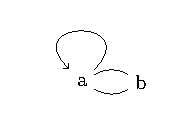
\includegraphics[scale=2]{images/3.pdf}
    \caption{Граф с одной петлёй и двумя кратными рёбрами.}
    \label{fig:3}
\end{figure}

\begin{definition}
    Два графа называются \textit{изоморфными}, если существует биекция между их множествами вершин и рёбер, уважающая отношение инцидентности.
\end{definition}

$v_1, v_2 \in V_1, \ e_1 \in E_1, \ f(v_1), f(v_2) \in V_2$ если вершины $v_1$ и $v_2$ были соединены ребром $e_1$, то их образы $f(v_1)$ и $f(v_2)$ соединены ребром $f(e_1)$.

\begin{figure}[h]
    \centering
    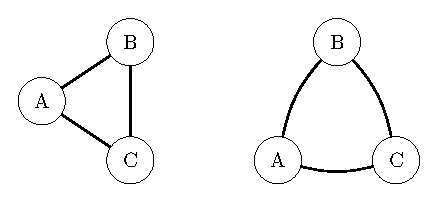
\includegraphics{images/4.pdf}
    \caption{Изоморфные графы.}
    \label{fig:4}
\end{figure}

\subsection{Топологическое описание графа}
\begin{definition}[Топологическое определение графа]
    Пусть дано множество (конечное) точек $V$, (конечное) множество отрезков $E$ и отображение $\partial$: (множество концов отрезков) $\to$ $V$. \textit{Графом}, определённым этими данными, назовём топологическое пространство, состоящее из множества точек $V$, называемых вершинами графа, множества внутренних точек отрезков $E$, называемых внутренними точками рёбер графа, на котором задана фактор-топология. Отношение эквивалентности: вершина $v$ лежит в том же классе эквивалентности, что и концы рёбер, которые в неё переходят.
\end{definition}

\cite{thebest}: В теории графов принята следующая терминология:
\begin{enumerate}
    \item если $v \in \partial(e)$, то говорят, что вершина $v$ и ребро $e$ \textit{инцидентны};
    \item если $\partial(e) = \left\{v,w\right\}$, то говорят, что вершины $v$ и $w$ \textit{смежны}, или же, что они соединены ребром $e$;
    \item рёбра $e, e'$ называются \textit{смежными}, если $\partial(e) \cap \partial(e') \neq \emptyset$;
    \item ребро, иницидентное ровно одной вершине, называется \textit{петлёй};
    \item если некоторой паре вершин инцидентно несколько рёбер, то все эти рёбра называются \textit{кратными};
    \item если некоторой вершине инцидентно несколько петель, то все эти петли также называются \textit{кратными}. [Конец цитирования]
\end{enumerate}


$v \in V, \ \partial^{-1}(v): A \sim B \Leftrightarrow A, B \in \partial^{-1}(v), \ A \sim B \sim v$.

\begin{definition}
    Графы называются \textit{гомеоморфными}, если они гомеоморфны как топологические пространства.
\end{definition}

\begin{figure}[h]
    \centering
    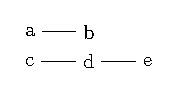
\includegraphics[scale=2]{images/5.pdf}
    \caption{Гомеорморфные, но не изоморфные графы.}
    \label{fig:5}
\end{figure}

\begin{definition}
    Непрерывное отображение графа $\Gamma$ в топологическое пространство $X$ называется \textit{вложением}, если при этом отображение $\Gamma$ и его образ гомеоморфны (никакие две различные точки не переходят в одну).
\end{definition}

\begin{figure}[h]
    \centering
    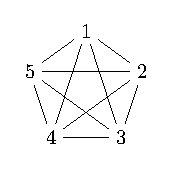
\includegraphics[scale=2]{images/6.pdf}
    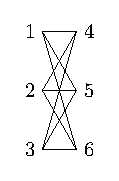
\includegraphics[scale=2]{images/7.pdf}
    \caption{$K_5$ и $K_{3,3}$ не являются планарными.}
    \label{fig:6}
\end{figure}

\begin{definition}[Вне лекций]
    Граф без петель и кратных рёбер называется \textit{простым}.
\end{definition}

\begin{definition}
    Граф, для которого существует его вложение в плоскость, называется \textit{планарным}.
\end{definition}

\begin{definition}
    Планарный граф вместе с вложением в плоскость называется \textit{плоским}.
\end{definition}

\begin{definition}[Вне лекций]
    $K_n$ — полный граф на $n$ вершинах, то есть граф, каждые две вершины которого соединены ребром.

    $K_{m,n}$ — двудольный граф, то есть граф, все вершины которого можно разбить на две группы так, что каждое ребро графа соединяет вершину из первой группы с вершиной из второй группы, при этом вершины из одной группы не имеют общих рёбер.
\end{definition}

\begin{figure}[h]
    \centering
    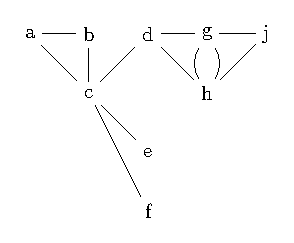
\includegraphics[scale=2]{images/8.pdf}
    \caption{Имеется пять областей, на которые разбивается плоскость.}
    \label{fig:8}
\end{figure}

\begin{theorem}
    Для связного плоского графа $B - P + \Gamma = 2$, где $\Gamma$ — количество областей, на которые граф разбивает плоскость.
\end{theorem}

\begin{theorem}[$\bigstar$]
    Для любого планарного графа существует его вложение в плоскость такое, что образ любого ребра является ломаной с конечным числом звеньев.
\end{theorem}

Свойства непрырывных кривых:

\begin{lemma}
    Образ $\gamma: [a,b] \to \R^2$ непрерывной кривой — замкнутое подмножество плоскости.
\end{lemma}
\begin{proof}
    $\left[a,b\right]$ — компакт $\Rightarrow$ образ его — компакт. $\R^2$ — хаусдорфово $\Rightarrow$ компакт замкнут в хаусдорфовом пространстве.

    \noindent \textit{Адаптированное доказательство из \cite{oshemkov}:} Возьмём точку $P$, которая не принадлежит образу кривой $\gamma$. Докажем, что существует такая окрестность $U$ этой точки $P$, что $U$ не пересекается с образом $\gamma$.

    Рассмотрим вспомогательную функцию $f$ на $[a,b]$, которая будет обозначать расстояние от точки $P$ до образа кривой. $f$ непрерывна $\Rightarrow$ достигает минимума $c > 0$ (т.к. $P$ не лежит в $\gamma$). Рассмотрим тогда круг радиуса $c / 2$ с центром в $P$. Получим окрестность $U_{P, c/2}$, которая не пересекается с образом $\gamma$.
\end{proof}

Сюда рисунок №6

\begin{lemma}
    $\Omega$ — замкнутое подмножество $\R^2$, $\gamma(t)$ — непрерывная кривая, $\gamma: [0,1] \to \R^2, \ \gamma(0) = A \notin \Omega, \ \gamma(1) = B \in \Omega \Rightarrow \exists t_0 \in  [0,1]: \ \gamma(t_0) \in \Omega, \ \forall t < t_0 \ \gamma(t) \notin \Omega$.
\end{lemma}
\begin{proof}
    Рассмотрим $T: \left\{
        \tau \in [0,1]: \ \forall t \in [0, \tau): \ \gamma(t) \notin \Omega
    \right\}$ — не пусто (так как $0 \in T$) и ограничено.

    Так как множество $T$ не пусто и ограничено, то можно сказать, что существует $\sup{T} = c$, более того, $c \neq 1$, т.к. $\gamma(1) = B \in \Omega$ по условию.

    Если $\gamma(c) = C \notin \Omega$, то существует окрестность $U$ точки $C$ такая, что $U \cap A = \emptyset$ (воспользовались замкнутостью множества $\Omega$).

    Так как $\gamma$ — непрерывная кривая, то существует окрестность $V = (c - \epsilon, c + \epsilon)$ такая, что $\gamma(V) \in U$, то есть $\forall t \in (c - \epsilon, c + \epsilon): \gamma(t) \notin \Omega \Rightarrow c \neq \sup{T}$ — противоречие, значит, $C \in \Omega$.
    
    В качестве $t_0$ возьмём $c$.

    (В исходнике есть наброски прямо с лекции)
    %$U$ — окрестность точки $A$: $U \cap \Omega = \emptyset \ \exists \tau_0: \ \gamma(t) \in U \Rightarrow t \in [0, \tau_0) \ \gamma(t) \notin \Omega, 0 \leq t < \tau_0$.
    %$\sup{\tau} = t_0$. Пусть $\gamma(t_0) \notin \Omega$, тогда существует $V$ окрестность $\gamma(t_0) \notin \Omega \Rightarrow \exists \delta \ \forall t \in (t_0 - \delta, t_0 + \delta), \ \gamma(t) \in V \Rightarrow \gamma(t) \notin \Omega, \ \gamma(t_0 + \frac{\delta}{2}) \notin \Omega \Rightarrow t_0$ — не супремум.
\end{proof}

\begin{proof}[Доказательство $\bigstar$]
    Пока не готово, можете посмотреть у Ошемкова \cite{oshemkov}.
    % Шаг 1. Удалим из графа петли.
    
    % Шаг 2. Сюда рисунок №7. Для каждой вершины рассмотрим окрестность такую, что она не пересекается с рёбрами графа, НЕ инцидентными данной вершине, и другими вершинами. Рассмотрим замкнутые окрестности вершин в два раза меньшего радиуса.

    % Шаг 3. Исправляем вложение в окрестности вершины и добавим обратно петли. Сюда рисунок №8

    % Шаг 4. Сюда рисунок №9.
\end{proof}

% конец третьей лекции